\documentclass[twoside]{book}

% Packages required by doxygen
\usepackage{fixltx2e}
\usepackage{calc}
\usepackage{doxygen}
\usepackage[export]{adjustbox} % also loads graphicx
\usepackage{graphicx}
\usepackage[utf8]{inputenc}
\usepackage{makeidx}
\usepackage{multicol}
\usepackage{multirow}
\PassOptionsToPackage{warn}{textcomp}
\usepackage{textcomp}
\usepackage[nointegrals]{wasysym}
\usepackage[table]{xcolor}

% Font selection
\usepackage[T1]{fontenc}
\usepackage[scaled=.90]{helvet}
\usepackage{courier}
\usepackage{amssymb}
\usepackage{sectsty}
\renewcommand{\familydefault}{\sfdefault}
\allsectionsfont{%
  \fontseries{bc}\selectfont%
  \color{darkgray}%
}
\renewcommand{\DoxyLabelFont}{%
  \fontseries{bc}\selectfont%
  \color{darkgray}%
}
\newcommand{\+}{\discretionary{\mbox{\scriptsize$\hookleftarrow$}}{}{}}

% Page & text layout
\usepackage{geometry}
\geometry{%
  a4paper,%
  top=2.5cm,%
  bottom=2.5cm,%
  left=2.5cm,%
  right=2.5cm%
}
\tolerance=750
\hfuzz=15pt
\hbadness=750
\setlength{\emergencystretch}{15pt}
\setlength{\parindent}{0cm}
\setlength{\parskip}{3ex plus 2ex minus 2ex}
\makeatletter
\renewcommand{\paragraph}{%
  \@startsection{paragraph}{4}{0ex}{-1.0ex}{1.0ex}{%
    \normalfont\normalsize\bfseries\SS@parafont%
  }%
}
\renewcommand{\subparagraph}{%
  \@startsection{subparagraph}{5}{0ex}{-1.0ex}{1.0ex}{%
    \normalfont\normalsize\bfseries\SS@subparafont%
  }%
}
\makeatother

% Headers & footers
\usepackage{fancyhdr}
\pagestyle{fancyplain}
\fancyhead[LE]{\fancyplain{}{\bfseries\thepage}}
\fancyhead[CE]{\fancyplain{}{}}
\fancyhead[RE]{\fancyplain{}{\bfseries\leftmark}}
\fancyhead[LO]{\fancyplain{}{\bfseries\rightmark}}
\fancyhead[CO]{\fancyplain{}{}}
\fancyhead[RO]{\fancyplain{}{\bfseries\thepage}}
\fancyfoot[LE]{\fancyplain{}{}}
\fancyfoot[CE]{\fancyplain{}{}}
\fancyfoot[RE]{\fancyplain{}{\bfseries\scriptsize Generated by Doxygen }}
\fancyfoot[LO]{\fancyplain{}{\bfseries\scriptsize Generated by Doxygen }}
\fancyfoot[CO]{\fancyplain{}{}}
\fancyfoot[RO]{\fancyplain{}{}}
\renewcommand{\footrulewidth}{0.4pt}
\renewcommand{\chaptermark}[1]{%
  \markboth{#1}{}%
}
\renewcommand{\sectionmark}[1]{%
  \markright{\thesection\ #1}%
}

% Indices & bibliography
\usepackage{natbib}
\usepackage[titles]{tocloft}
\setcounter{tocdepth}{3}
\setcounter{secnumdepth}{5}
\makeindex

% Hyperlinks (required, but should be loaded last)
\usepackage{ifpdf}
\ifpdf
  \usepackage[pdftex,pagebackref=true]{hyperref}
\else
  \usepackage[ps2pdf,pagebackref=true]{hyperref}
\fi
\hypersetup{%
  colorlinks=true,%
  linkcolor=blue,%
  citecolor=blue,%
  unicode%
}

% Custom commands
\newcommand{\clearemptydoublepage}{%
  \newpage{\pagestyle{empty}\cleardoublepage}%
}

\usepackage{caption}
\captionsetup{labelsep=space,justification=centering,font={bf},singlelinecheck=off,skip=4pt,position=top}

%===== C O N T E N T S =====

\begin{document}

% Titlepage & ToC
\hypersetup{pageanchor=false,
             bookmarksnumbered=true,
             pdfencoding=unicode
            }
\pagenumbering{roman}
\begin{titlepage}
\vspace*{7cm}
\begin{center}%
{\Large My Project }\\
\vspace*{1cm}
{\large Generated by Doxygen 1.8.11}\\
\end{center}
\end{titlepage}
\clearemptydoublepage
\tableofcontents
\clearemptydoublepage
\pagenumbering{arabic}
\hypersetup{pageanchor=true}

%--- Begin generated contents ---
\chapter{File Index}
\section{File List}
Here is a list of all files with brief descriptions\+:\begin{DoxyCompactList}
\item\contentsline{section}{\hyperlink{Lab1_8c}{Lab1.\+c} }{\pageref{Lab1_8c}}{}
\end{DoxyCompactList}

\chapter{File Documentation}
\hypertarget{RPG_8cpp}{}\section{R\+P\+G.\+cpp File Reference}
\label{RPG_8cpp}\index{R\+P\+G.\+cpp@{R\+P\+G.\+cpp}}
{\ttfamily \#include $<$iostream$>$}\\*
{\ttfamily \#include $<$cstdlib$>$}\\*
{\ttfamily \#include $<$ctime$>$}\\*
Include dependency graph for R\+P\+G.\+cpp\+:
\nopagebreak
\begin{figure}[H]
\begin{center}
\leavevmode
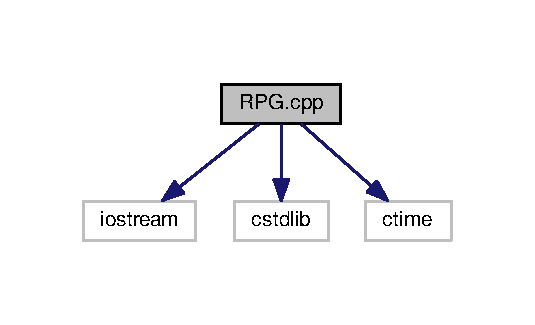
\includegraphics[width=257pt]{RPG_8cpp__incl}
\end{center}
\end{figure}
\subsection*{Functions}
\begin{DoxyCompactItemize}
\item 
int \hyperlink{RPG_8cpp_ae66f6b31b5ad750f1fe042a706a4e3d4}{main} ()
\end{DoxyCompactItemize}


\subsection{Function Documentation}
\index{R\+P\+G.\+cpp@{R\+P\+G.\+cpp}!main@{main}}
\index{main@{main}!R\+P\+G.\+cpp@{R\+P\+G.\+cpp}}
\subsubsection[{\texorpdfstring{main()}{main()}}]{\setlength{\rightskip}{0pt plus 5cm}int main (
\begin{DoxyParamCaption}
{}
\end{DoxyParamCaption}
)}\hypertarget{RPG_8cpp_ae66f6b31b5ad750f1fe042a706a4e3d4}{}\label{RPG_8cpp_ae66f6b31b5ad750f1fe042a706a4e3d4}

\begin{DoxyCode}
8 \{
9   \textcolor{keywordtype}{int} choice;
10   \textcolor{keywordtype}{int} mhp, hp, i, init, atk, def, matk, mdef, hurt, mhurt, agi, magi;
11   atk = 10;
12   def = 15;
13   agi = 5;
14   matk = 10;
15   mdef = 15;
16   magi = 5;
17   
18   srand((\textcolor{keywordtype}{unsigned})time(0));
19   init = rand()%2+1;
20   mhp = rand()%50 + 60;
21   hp = rand()%20 + 80;
22   \textcolor{keywordflow}{if} (init == 1) \{
23   cout<<\textcolor{stringliteral}{"You start.\(\backslash\)n"};
24   \textcolor{keywordflow}{while} (hp > 0 || mhp > 0) \{
25     cout<<\textcolor{stringliteral}{"What do you want to do?\(\backslash\)n1 - Fierce Attack\(\backslash\)n2 - Lithe Attack\(\backslash\)n3 - Defensive moves\(\backslash\)n"};
26      \textcolor{keywordflow}{do}\{cin>>choice;\}\textcolor{keywordflow}{while}(choice>3 || choice<1);
27     \textcolor{keywordflow}{switch} (choice) \{
28       \textcolor{keywordflow}{case} 1:
29         atk = rand()%20+10;
30     def = rand()%10+10;
31     agi = rand()%5;
32     \textcolor{keywordflow}{break};
33       \textcolor{keywordflow}{case} 2:
34         atk = rand()%5+10;
35     def = rand()%10+10;
36     agi = rand()%15;
37         \textcolor{keywordflow}{break};
38       \textcolor{keywordflow}{case} 3:
39         atk = rand()%10+10;
40     def = rand()%20+10;
41     agi = rand()%5;
42     \textcolor{keywordflow}{break};
43     \}
44     choice = rand()%3;
45     \textcolor{keywordflow}{switch} (choice) \{
46       \textcolor{keywordflow}{case} 1:
47         matk = rand()%20+10;
48     mdef = rand()%10+10;
49     magi = rand()%5;
50     \textcolor{keywordflow}{break};
51       \textcolor{keywordflow}{case} 2:
52         matk = rand()%5+10;
53     mdef = rand()%10+10;
54     magi = rand()%15;
55         \textcolor{keywordflow}{break};
56       \textcolor{keywordflow}{case} 3:
57         matk = rand()%10+10;
58     mdef = rand()%20+10;
59     magi = rand()%5;
60     \textcolor{keywordflow}{break};
61     \}
62 
63 \textcolor{comment}{//Här dör folk o sånt}
64     mhurt = (atk - magi) - (mdef/atk);
65     \textcolor{keywordflow}{if} (mhurt < 0) \{
66       mhurt = 0;
67     \}
68     mhp = mhp - mhurt;
69     cout<<\textcolor{stringliteral}{"You did "}<<mhurt<<\textcolor{stringliteral}{" damage to the monster!\(\backslash\)n"};
70     cin.get();
71 \textcolor{comment}{//Specielt här}
72     \textcolor{keywordflow}{if} (mhp < 1) \{
73       cout<<\textcolor{stringliteral}{"You killed the beast!! You won with "}<<hp<<\textcolor{stringliteral}{" hp left.\(\backslash\)n"};
74       cin.get();
75       \textcolor{keywordflow}{return} 0;
76       \}
77     cout<<\textcolor{stringliteral}{"The monster now have "}<<mhp<<\textcolor{stringliteral}{" hp left.\(\backslash\)n"};
78     hurt = (matk - agi) - (def/matk);
79     \textcolor{keywordflow}{if} (hurt < 0) \{
80       hurt = 0;
81     \}
82     hp = hp - hurt;
83     cout<<\textcolor{stringliteral}{"The monster hit you for "}<<hurt<<\textcolor{stringliteral}{" damage.\(\backslash\)n"};
84 \textcolor{comment}{//Och här.}
85     \textcolor{keywordflow}{if} (hp < 1) \{
86       cout<<\textcolor{stringliteral}{"You died. The beast still has "}<<mhp<<\textcolor{stringliteral}{" hp left.\(\backslash\)n"};
87       cin.get();
88       \textcolor{keywordflow}{return} 0;
89       \}
90 cout<<\textcolor{stringliteral}{"You now have "}<<hp<<\textcolor{stringliteral}{" hp left.\(\backslash\)n\(\backslash\)n"};
91      \}
92      \}
93 
94 \textcolor{comment}{//Om monstret startar.}
95   \textcolor{keywordflow}{else} \{
96   cout<<\textcolor{stringliteral}{"Monster start.\(\backslash\)n"};
97     \textcolor{keywordflow}{while} (hp > 0 || mhp > 0) \{
98     choice = rand()%3;
99     \textcolor{keywordflow}{switch} (choice) \{
100       \textcolor{keywordflow}{case} 1:
101         matk = rand()%20+10;
102     mdef = rand()%10+10;
103     magi = rand()%5;
104     \textcolor{keywordflow}{break};
105       \textcolor{keywordflow}{case} 2:
106         matk = rand()%5+10;
107     mdef = rand()%10+10;
108     magi = rand()%15;
109         \textcolor{keywordflow}{break};
110       \textcolor{keywordflow}{case} 3:
111         matk = rand()%10+10;
112     mdef = rand()%20+10;
113     magi = rand()%5;
114     \textcolor{keywordflow}{break};
115     \}
116 \textcolor{comment}{//Monstret börjar!! han slår till direkt.}
117     hurt = (matk - agi) - (def/matk);
118     \textcolor{keywordflow}{if} (hurt < 0) \{
119       hurt = 0;
120     \}
121     hp = hp - hurt;
122     cout<<\textcolor{stringliteral}{"The monster hit you for "}<<hurt<<\textcolor{stringliteral}{" damage.\(\backslash\)n"};
123 \textcolor{comment}{//Oooooh, gotta hurt!}
124     \textcolor{keywordflow}{if} (hp < 1) \{
125       cout<<\textcolor{stringliteral}{"You died. The beast still has "}<<mhp<<\textcolor{stringliteral}{" hp left.\(\backslash\)n"};
126       cin.get();
127       \textcolor{keywordflow}{return} 0;
128       \}
129  cout<<\textcolor{stringliteral}{"You now have "}<<hp<<\textcolor{stringliteral}{" hp left.\(\backslash\)n\(\backslash\)n"};
130     cout<<\textcolor{stringliteral}{"What do you want to do?\(\backslash\)n1 - Fierce Attack\(\backslash\)n2 - Lithe Attack\(\backslash\)n3 - Defensive moves\(\backslash\)n"};
131      \textcolor{keywordflow}{do}\{cin>>choice;\}\textcolor{keywordflow}{while}(choice>3 || choice<1);
132     \textcolor{keywordflow}{switch} (choice) \{
133       \textcolor{keywordflow}{case} 1:
134         atk = rand()%20+10;
135     def = rand()%10+10;
136     agi = rand()%5;
137     \textcolor{keywordflow}{break};
138       \textcolor{keywordflow}{case} 2:
139         atk = rand()%5+10;
140     def = rand()%10+10;
141     agi = rand()%15;
142         \textcolor{keywordflow}{break};
143       \textcolor{keywordflow}{case} 3:
144         atk = rand()%10+10;
145     def = rand()%20+10;
146     agi = rand()%5;
147     \textcolor{keywordflow}{break};
148         \}
149 
150 
151 \textcolor{comment}{//Här kan han dö.}
152     mhurt = (atk - magi) - (mdef/atk);
153     \textcolor{keywordflow}{if} (mhurt < 0) \{
154       mhurt = 0;
155     \}
156     mhp = mhp - mhurt;
157     cout<<\textcolor{stringliteral}{"You did "}<<mhurt<<\textcolor{stringliteral}{" damage to the monster!\(\backslash\)n"};
158     cin.get();
159 \textcolor{comment}{//Eller typ här:}
160     \textcolor{keywordflow}{if} (mhp < 1) \{
161       cout<<\textcolor{stringliteral}{"You killed the beast!! You won with "}<<hp<<\textcolor{stringliteral}{" hp left.\(\backslash\)n"};
162       cin.get();
163       \textcolor{keywordflow}{return} 0;
164       \}
165     cout<<\textcolor{stringliteral}{"The monster now have "}<<mhp<<\textcolor{stringliteral}{" hp left.\(\backslash\)n"};
166   \} \} \}\end{DoxyCode}

%--- End generated contents ---

% Index
\backmatter
\newpage
\phantomsection
\clearemptydoublepage
\addcontentsline{toc}{chapter}{Index}
\printindex

\end{document}
